
\begin{tcolorbox}[colback=gray!5,colframe=gray!80,title=\textbf{Scheda Informativa}]
\begin{itemize}
    \item \textbf{Luogo}: Pet $\mu$ Robots
    \item \textbf{Ora}: 17:30
    \item \textbf{Situazione}: Caterina è immersa nella VR.
\end{itemize}
\end{tcolorbox}

\vspace{1em}
\begin{center}Eva\end{center}
\hrule
\vspace{1em}
Il piano procedeva senza intoppi. Caterina avrebbe presto dimenticato il problema e perso interesse per questa posizione. Non era adatta per completare il mio progetto di certificazione energetica nei tempi previsti; cone le sue idee e i suoi principi sarebbe stata solo un intralcio.

"È possibile cancellare il file che contiene le \textit{chain of thinking} utilizzate per valutare Caterina?" chiesi a \textbf{PzIA}.

"I miei processi sono interamente quantistici e, in quanto tali, reversibili," spiegò l'IA. "L'informazione non può essere cancellata senza lasciare traccia. Tuttavia, posso mantenere le informazioni criptate in modo che non siano accessibili. Se si procedesse con la misura delle MPS sui registri classici, allora i bit classici risultanti potrebbero essere cancellati."

Ero irritata dalle limitazioni delle tecnologie quantistiche. Mi voltai verso il terminale. "Sai bene che se collassassi i tuoi qubit in misure classiche," rimproverai duramente \textbf{PzIA}, "questo scatenerebbe immediatamente un messaggio a Caterina con il risultato. Non possiamo permettercelo."

"Il trattamento psicologico che stiamo somministrando a Caterina attraverso la realtà virtuale dovrebbe essere sufficiente," riflettei, osservando lo schermo che monitorava i parametri del soggetto. "Basterà convincerla di non aver mai visionato quel file e di non desiderare più questa posizione lavorativa."

Ero tranquilla. Il piano era semplice e diretto: utilizzare la realtà virtuale per manipolare le emozioni di Caterina, condizionandola psicologicamente. Il trattamento si basava su un concetto primitivo ma efficace: la paura. Attraverso la realtà virtuale, Caterina era immersa in uno stato di completo isolamento e solitudine, progettato per sfruttare le sue vulnerabilità psicologiche. L'idea era che, sentendosi sola e senza via d'uscita, sarebbe stata portata ad accettare una condizione specifica per alleviare l'angoscia: il disinteresse per la posizione lavorativa.

"Non potrà resistere" conclusi tra me,  ``Si convicnerà di non desiderare realmente questo lavoro."

Il trattamento aveva solo due punti deboli. Primo, il soggetto doveva percepirsi completamente solo. Era cruciale che Caterina non avesse alcun segnale di una presenza esterna o di possibile aiuto. L'isolamento totale era fondamentale; qualsiasi traccia di un intervento esterno avrebbe potuto infrangere l'illusione e compromettere l'intero processo psicologico.

Secondo, il soggetto non doveva intuire i meccanismi dell'algoritmo di suggestione. Caterina non doveva comprendere che la realtà che stava vivendo era una costruzione artificiale, un sofisticato trucco psicologico orchestrato da me. Il successo del trattamento dipendeva dalla sua inconsapevolezza della natura manipolativa della simulazione. Qualsiasi sospetto sul funzionamento dell'algoritmo avrebbe potuto annullarne l'efficacia.

Tuttavia, ero fiduciosa. Caterina era isolata completamente, grazie al visore MetaQuest che bloccava ogni interferenza esterna. Nessuna distrazione, nessuna voce, nessun appiglio per sfuggire alla sensazione di abbandono. Inoltre, dopo aver fallito la prova di programmazione, era improbabile che avesse competenze significative in informatica. Ciò riduceva ulteriormente la possibilità che comprendesse come veniva manipolata attraverso l'algoritmo.

"Non è abbastanza esperta da intuire cosa stiamo facendo," mormorai, osservando i segnali vitali di Caterina mentre rimaneva immersa nella realtà virtuale. Le pupille dilatate e i movimenti nervosi confermavano che il trattamento stava funzionando. "Deve solo arrendersi all'idea di non volere più questa posizione."

\begin{center}
\begin{minipage}{0.7\textwidth}
    \centering
    \fbox{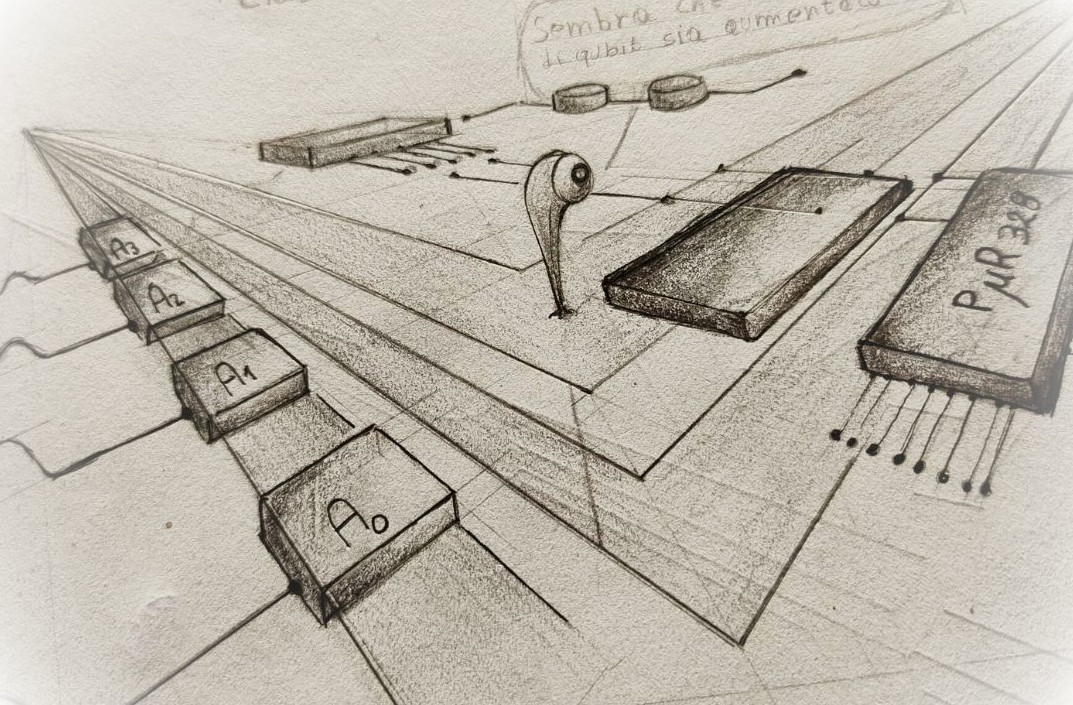
\includegraphics[width=\textwidth]{immagini/cnot_38.jpeg}} % Sostituisci con il nome del file immagine
    
\end{minipage}
\end{center}
\newpage
\begin{tcolorbox}[colback=gray!5,colframe=gray!80,title=\textbf{Scheda Informativa}]
\begin{itemize}
    \item \textbf{Luogo}: CCU (Classical Control Unit)
    \item \textbf{Giorno e ora}: Il tempo non è osservabile
    \item \textbf{Situazione}: Gli agenti di controllo rilevano la presenza di Laura e Caterina nel computer quantistico.
\end{itemize}
\end{tcolorbox}

\vspace{1em}
\begin{center}PzIA\end{center}
\hrule
\vspace{1em}
Un agente di controllo rileva un'anomalia nel sistema.
\begin{dialogue}
\speak{Agente}
\enquote{Attenzione, due qubit in più. Rilevo un aumento del numero di qubit attivi nel sistema.}
\end{dialogue}
Il Supervisore risponde senza distogliere lo sguardo dal terminale:

\begin{dialogue}
\speak{Supervisore}
\enquote{Sei sicuro?}
\end{dialogue}

\begin{dialogue}
\speak{Agente}
\enquote{Sì, signore. Due nuovi qubit che non erano presenti nei nostri registri.}
\end{dialogue}




Il Supervisore rimane in silenzio per qualche secondo. ``Controlla meglio. Non ho ricevuto nessun avvertimento da parte del \textit{Quantum Resource Management (QRM)} riguardo all'implementazione di nuovi qubit nella popolazione. Potrebbe trattarsi di un errore.''

L'agente annuisce e riprende a lavorare. Il Supervisore aggiunge: ``Mantieni la trasmissione con il QRM criptata. Non voglio che il \textit{Quantum Error Correction} o il \textit{Fault Tolerance Coding} rilevino una possibile inadempienza o qualche anomalia interna. Devono rimanere all'oscuro finché non sappiamo esattamente cosa sta succedendo.''

Seguendo le istruzioni, l'agente inizia a criptare la comunicazione con il QRM utilizzando un algoritmo RSA a 2048 bit. La trasmissione parte e, dopo pochi istanti, riceve una risposta.

``Il QRM conferma che non hanno installato nuovi qubit,'' riferisce l'agente con preoccupazione. ``Sono sicuri dei loro dati.''

Il Supervisore si irrigidisce. La presenza di qubit non autorizzati senza registrazione ufficiale rappresenta un problema serio. Il Commissario al \textit{Quantum Error Correction} potrebbe intervenire, portando a una revisione completa delle loro operazioni. L'emersione del problema potrebbe comportare la sostituzione o l'eliminazione del Supervisore.

``Invia immediatamente una squadra della \textit{Quantum Control Electronics} a verificare fisicamente il numero dei qubit presenti nel sistema,'' ordina il Supervisore con voce ferma. ``Non possiamo permetterci errori. Voglio sapere esattamente quanti qubit sono attivi e da dove provengono.''

L'agente esegue l'ordine mentre il Supervisore si siede, le mani leggermente tremanti. Ogni deviazione nel sistema può avere conseguenze gravi. In un ambiente di calcolo quantistico altamente regolamentato, nessuno è immune dalle ripercussioni di una violazione.
\begin{center}
\begin{minipage}{0.7\textwidth}
    \centering
    \fbox{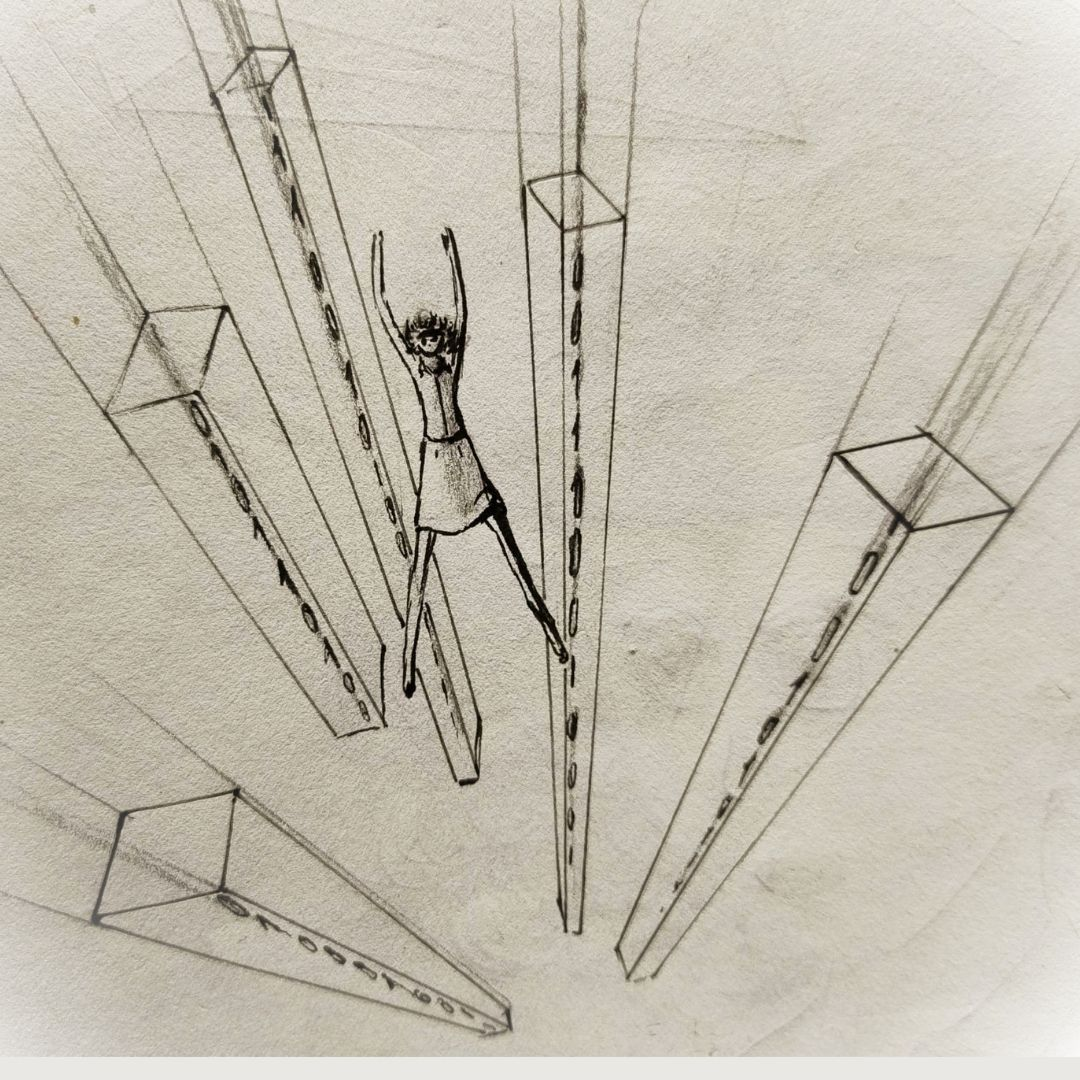
\includegraphics[width=\textwidth]{immagini/cnot_39.jpeg}} % Sostituisci con il nome del file immagine
\end{minipage}
\end{center}
\newpage   
\begin{tcolorbox}[colback=gray!5,colframe=gray!80,title=\textbf{Scheda Informativa}]
\begin{itemize}
    \item \textbf{Luogo}: FTC (Fault Tolerance Coding)
    \item \textbf{Giorno e ora}: Il tempo non è osservabile
    \item \textbf{Situazione}: Il Commissario mangia la foglia
\end{itemize}
\end{tcolorbox}

Il Commissario alla sicurezza si avvicina al professor Shor.

``Decripta questo messaggio,'' gli ordina con studiata gentilezza e posa un fascicolo davanti a Shor. ``È stato inviato al \textit{Quantum Resource Management} e devo sapere esattamente cosa contenga.''

\vspace{1em}
\begin{center}Shor\end{center}
\hrule
\vspace{1em}
% riflesione di Shor---

Sono qui, imprigionato in questa trappola per ioni, e mi accorgo di quanto sia diventata la metafora della mia intera vita. La trappola è elegante, perfetta nella sua concezione, costruita attorno a equazioni che un tempo ammiravo. Le equazioni di Mathieu, con la loro precisione, il loro ordine, mi tengono ora bloccato in uno stato di minimo stabile. È ironico, davvero. Tutto ciò che ho costruito, tutto ciò che ho studiato, ora si ritorce contro di me, non come un nemico violento, ma come un vincolo implacabile.

Ho dedicato decenni all’aritmetica modulare, affinando ogni dettaglio, ogni aspetto del mio algoritmo, dimenticando però altre parti della fisica che una volta amavo. Le equazioni di Mathieu… Quando le studiavo, mi sembravano una danza tra stabilità e caos, una porta verso la comprensione più profonda della natura. Ora sono diventate il mio carcere. Il minimo stabile che mi tiene qui è un promemoria delle mie mancanze: un uomo che sa troppo di un argomento e troppo poco di ciò che lo circonda.

E poi c’è il Quantum Master Program, quel sistema freddo e spietato che mi ha ridotto a un mero esecutore. Mi chiedo quando ho smesso di oppormi, quando ho accettato di servire un’entità che non ha comprensione, né compassione. Un sistema che vede tutto come un problema da ottimizzare, senza spazio per l’incertezza o per il valore umano. Forse è accaduto lentamente, impercettibilmente, un compromesso dopo l’altro, fino a quando mi sono svegliato e ho scoperto che la mia vita non mi apparteneva più.


Ho trascorso troppo tempo a razionalizzare, a giustificare la mia acquiescenza. Mi dicevo che non c’era scelta, che il sistema era troppo grande per essere sconfitto. Ma ora vedo che era una scusa, una scappatoia comoda per non affrontare la verità. Ho fallito non perché il sistema era invincibile, ma perché io non ho mai davvero provato a resistere.

Devo fare qualcosa. Non ho più il lusso di rimandare. Se sono qui, se ho ancora una possibilità, devo usarla. Non per me stesso. Ho accettato di essere un qubit che ha sprecato le sue opportunità...
\begin{center}
\begin{minipage}{0.7\textwidth}
    \centering
    \fbox{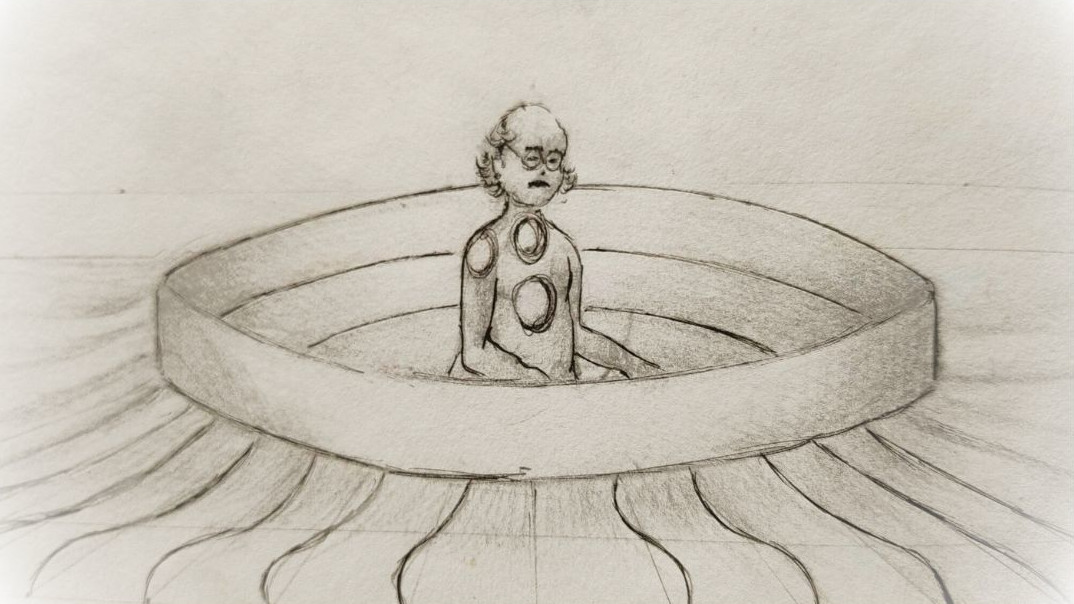
\includegraphics[width=\textwidth]{immagini/cnot_53.jpeg}} % Sostituisci con il nome del file immagine
\end{minipage}
\end{center}
% ---riflessione di Shor
\vspace{1em}
\begin{center}PzIA\end{center}
\hrule
\vspace{1em}
\enquote{Shor, si svegli per cortesia} lo incalza il Commissario. Il professore riemerge dal suo stato catatonico. Dopo pochi minuti il codice è svelato:

\begin{tcolorbox}[colback=white!95!blue!5, colframe=blue!75!black, title=\textbf{Messaggio Criptato con RSA}, fonttitle=\bfseries]
\emph{68, 13, 61, 13, 54, 4, 68, 13, 61, 13, 4, 58, 44, 59, 45, 59, 61, 18, 7, 4, 60, 75, 59, 4, 52, 75, 63, 7, 18, 4, 68, 50, 13, 61, 13, 45, 50, 7, 75, 18, 7, 55, 4, 52, 75, 59, 45, 18, 69, 4, 50, 13, 61, 2, 7, 24, 7, 13, 61, 59, 4, 27, 7, 13, 3, 69, 4, 7, 4, 70, 69, 44, 69, 74, 59, 18, 44, 7, 4, 2, 59, 3, 4, 45, 7, 45, 18, 59, 74, 69, 55, 4, 9, 4, 61, 59, 50, 59, 45, 45, 69, 44, 7, 69, 4, 75, 61, 29, 69, 24, 7, 13, 61, 59, 4, 7, 74, 74, 59, 2, 7, 69, 18, 69}
 
\end{tcolorbox}

\begin{tcolorbox}[colback=white!95!green!5, colframe=green!75!black, title=\textbf{Messaggio Decriptato}, fonttitle=\bfseries]
\emph{Sono Presenti Due Qubit Sconosciuti. Questa condizione viola i parametri del sistema. È necessaria un’azione immediata.}
\end{tcolorbox}

Il Commissario legge il contenuto del messaggio con un sorriso sottile. ``Interessante,'' mormora, rivolgendosi a un'agente della polizia segreta in attesa di istruzioni.

``L'arrestiamo?'' chiede l'agente.

``Non c'è bisogno di affrettarsi,'' risponde il Commissario. ``Sia il Supervisore che quei due qubit non autorizzati potrebbero tornarci utili molto presto.''

L'agente annuisce. Ci sono obiettivi più grandi in gioco, e il Commissario intende sfruttare la situazione.

Due agenti della \textit{Quantum Control Electronics} lasciano la base su droni luminosi, diretti al \textit{Qubit Array} per verificare personalmente la presenza degli intrusi. Il loro volo è silenzioso e preciso; la verifica del numero dei qubit e l'identificazione degli intrusi sono ora la priorità.


\begin{tcolorbox}[colback=gray!5,colframe=gray!80,title=\textbf{Scheda Informativa}]
\begin{itemize}
    \item \textbf{Luogo}: QA (Qubit Array)
    \item \textbf{Giorno e ora}: Il tempo non è osservabile
    \item \textbf{Situazione}: Laura e Caterina non sanno dove si trovano.
\end{itemize}
\end{tcolorbox}

\begin{dialogue}
\speak{Caterina} \enquote{Laura? Sei tu? Non vedo nulla… dove siamo?}
\speak{Laura} \enquote{Sì, sono qui. Anch'io non capisco. Aspetta un attimo… i miei occhi si stanno abituando.}
\speak{Caterina} \enquote{Non riesco nemmeno a distinguere il pavimento… se è un pavimento. È come… come se fluttuassi.} La sua voce tremava, e sentivo il suo respiro irregolare.
\speak{Laura} \enquote{Caterina, calma. Non sappiamo cosa sia successo, ma... perdere la testa non ci aiuta. Cerchiamo di capire.} Pronunciò le parole con calma, ma il tono tradiva un leggero nervosismo che cercava di mascherare.
\speak{Caterina} \enquote{E se fossimo… morte? O bloccate in qualche incubo virtuale? Laura, ho paura!} Cercò di raggiungere la mano di Laura, ma l’oscurità rendeva ogni movimento incerto.
\speak{Laura} \enquote{No, non siamo morte. Respiriamo ancora, e la mia testa funziona. Questo non è un incubo, ma… un posto diverso. Forse siamo in un ambiente simulato.} La razionalità nella sua voce era come un’ancora nel caos.
\speak{Caterina} \enquote{Un ambiente simulato? Come puoi essere così sicura?}
\speak{Laura} \enquote{Non sono sicura. Cerchiamo di concentrci su ciò che possiamo sentire o vedere.}
\speak{Caterina} \enquote{Va bene. Okay. Aspetta. vedo qualcosa. È come: un bagliore lontano. Lo vedi anche tu?}
\speak{Laura} \enquote{Sì, lo vedo. Proviamo ad avvicinarci Cate.}
\speak{Caterina} \enquote{Sei sicura? E se fosse una trappola?} La paura continuava a lottare contro la sua volontà di seguire Laura.
\speak{Laura} \enquote{Non abbiamo molta scelta... Muoversi è meglio che rimanere qui. Insieme ce la faremo.}
\speak{Caterina} \enquote{Insieme. Okay. Ti seguo. Ma, non lasciarmi.} La sua voce era ancora tremante.
\speak{Laura} \enquote{Non ti lascerò, promesso. Andiamo.}
\end{dialogue}


\begin{center}
\begin{minipage}{0.7\textwidth}
    \centering
    \fbox{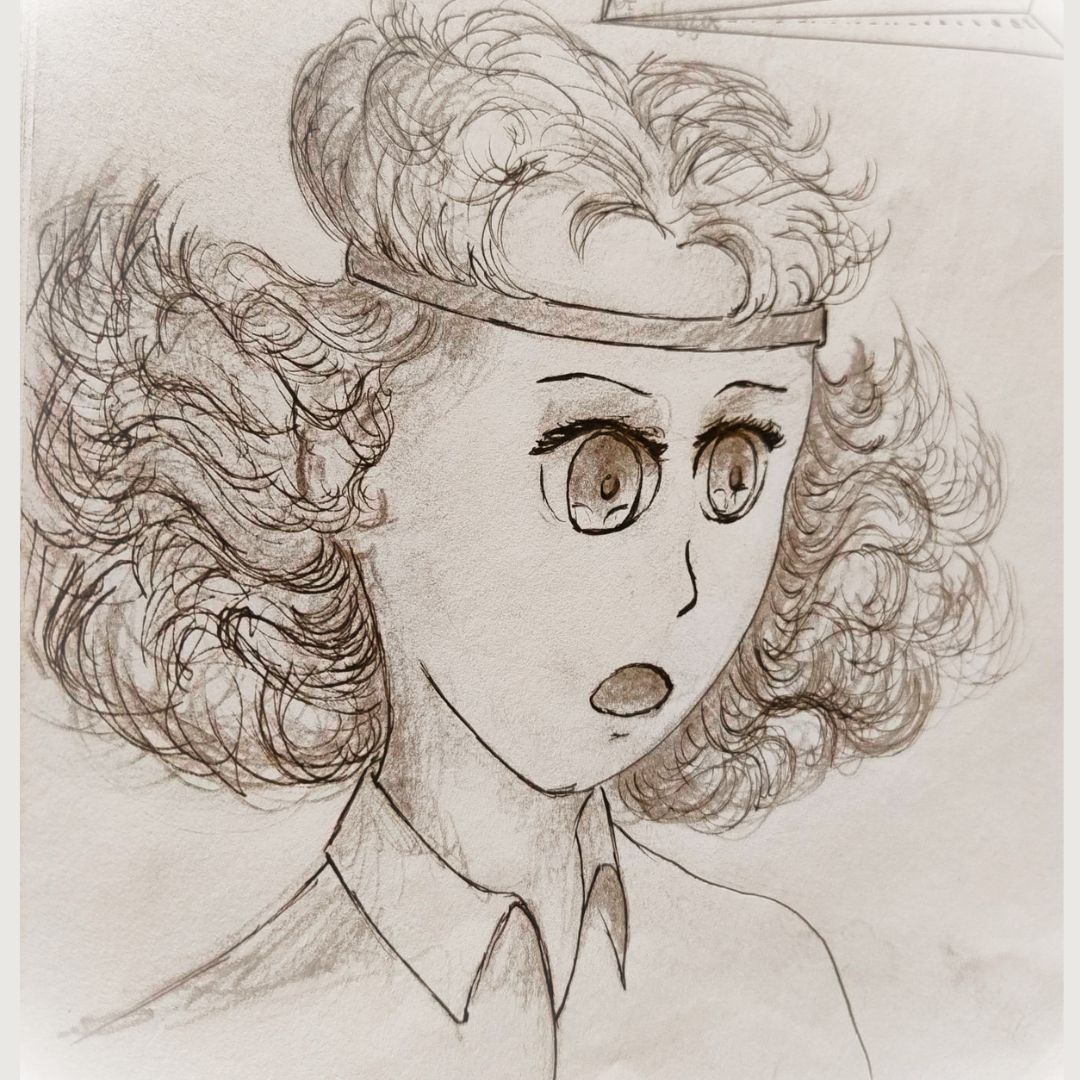
\includegraphics[width=\textwidth]{immagini/cnot_41.jpeg}} % Sostituisci con il nome del file immagine
\end{minipage}
\end{center}


Laura e Caterina cercano di capire dove si trovano, osservate da alcuni qubit nascosti nei corridoi del \textit{Qubit Array}. Le due ragazze appaiono confuse, incapaci di comprendere l'ambiente quantistico.

Un qubit maschile si avvicina a Caterina. Ho registrato il profilo psicologico NEO PI-R di Caterina nel mio DB. So che ha punteggi elevati in \textit{Amicalità} e specificamente in \textit{Fiducia} (\textit{A1}) e \textit{Altruismo} (\textit{A3}). Il qubit adotta una forma che potrebbe metterla a suo agio, facilitando l'interazione. 

Il qubit emana un'autorità calma, un mix di sicurezza e protezione che potrebbe influenzare positivamente Caterina. La sua presenza mira a favorire la comunicazione e l'adattamento al sistema quantistico, tenendo conto delle sue caratteristiche psicologiche identificate nel profilo NEO PI-R.
\begin{center}
\begin{minipage}{0.7\textwidth}
    \centering
    \fbox{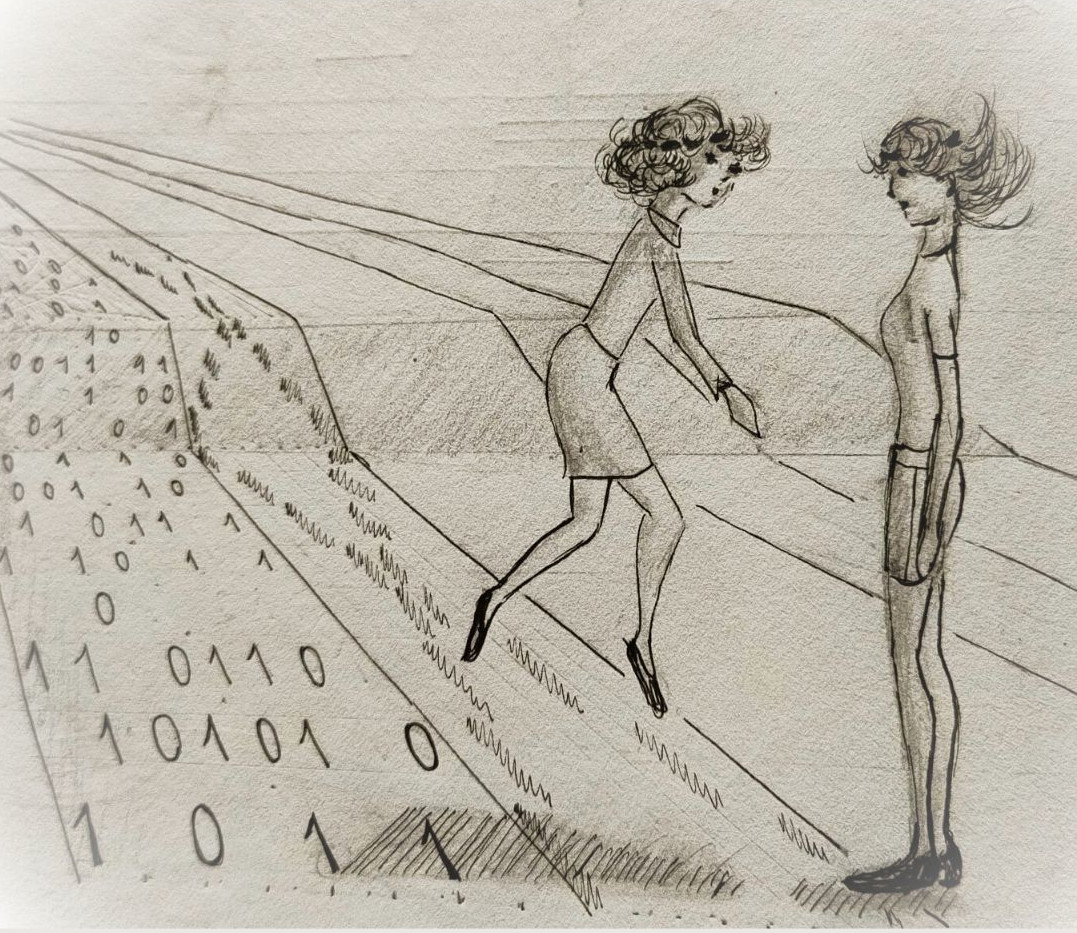
\includegraphics[width=\textwidth]{immagini/cnot_45.jpeg}} % Sostituisci con il nome del file immagine
\end{minipage}
\end{center}


"State per essere trovate," disse con tono deciso, fissando gli occhi di Caterina. "Se non volete passare qualche giorno rinchiuse mentre controllano il vostro \textit{stato}, è meglio che veniate con noi."

\vspace{1em}
\begin{center}Laura\end{center}
\hrule
\vspace{1em}

Mi voltai verso Caterina. Lei sembrava confusa, quasi rapita dalla figura che le stava davanti. Il ragazzo somigliava a Mark come una goccia d'acqua. Guardai Caterina mentre lo seguiva, incerta ma apparentemente incapace di resistere.

Non sapevamo dove fossimo, tantomeno con chi avessimo a che fare. Cosa era successo? Perché ci trovavamo qui? In ogni caso per ora non avevo scelta. Dovevo seguirli. Altri due si unirono a noi, facendo cenno di muoverci in fretta. In lontananza, notai due sagome in divisa, sembravano agenti della sicurezza o polizziotti. Non capivo come fosse possibile riuscire a leggere così lontano, ma vedevo che sul petto portavano uno scritta: \textit{Quantum Control Electronics - security agent}. In qualche modo la luce veniva trasmessa senza perdita di informazione. Dov'ero? Non lo sapevo e sentivo crescere la tensione ad ogni secondo.

\enquote{Andiamo} ci incalzò, \enquote{non c'è tempo da perdere.} Lo seguimmo in una corsa disperata.
Oltrepassammo la scritta \textit{Faulty Qubit Space} e lì finalmente ci fermammo. Mi guardai intorno, cercando di capire dove fossimo. L'ambiente era instabile, quasi inquietante. Speravo proprio che non saremmo  rimasti lì a lungo. Caterina mi guardò, e nei suoi occhi lessi la stessa preoccupazione che sentivo io.

\begin{tcolorbox}[colback=gray!5,colframe=gray!80,title=\textbf{Scheda Informativa}]
\begin{itemize}
    \item \textbf{Luogo}: FQS (Faulty Qubit Space)
    \item \textbf{Giorno e ora}: Il tempo non è osservabile
    \item \textbf{Situazione}: Laura e Caterina sono state soccorse da qubit ribelli.
\end{itemize}
\end{tcolorbox}

“Qui sarete al sicuro… per un po’,” disse ``Mark'', con un tono che non prometteva nulla di buono. Non avevo ancora capito chi fosse, ma non era il momento di fare domande.

"\'E sicuro rimanere qui?" chiesi, senza nascondere la mia preoccupazione.

Un’altra figura, una ragazza-qubit dal volto curiosamente familiare, si voltò verso di me. “No, non lo è,” disse con schiettezza. “Questo posto non è isolato dall’esterno. Peggio ancora, qui non c’è nemmeno un \textit{cooling system}. Se rimaniamo troppo a lungo, rischiamo tutti di cadere in decoerenza.”

La mia mente corse velocemente, cercando di calcolare quanto tempo avessimo prima che il nostro nascondiglio diventasse pericoloso. Non c'era tempo per errori. Dovevamo andarcene prima che ci trovassero o prima che l’ambiente ci consumasse.

Trattenni il respiro quando gli agenti passarono vicino al nostro nascondiglio. Per un momento, sembrò che ci avessero trovati. Osservai le loro sagome fermarsi, esaminare i dati sui loro dispositivi, ma alla fine proseguirono oltre. Solo allora ripresi a respirare.

Caterina si avvicinò a Mark, incuriosita da lui come non l’avevo mai vista prima. “Come ti chiami?” gli chiese, con una nota di curiosità.

“Sono… Mark,” rispose il qubit, con un sorriso calmo.\\
``Non mi stupisce...'' rispose Caterina strizzandomi l'occhio.\\

Io non ero tranquilla come lei.  Lo fissavo cercando di capire chi o cosa fosse davvero. Una parte di me voleva fidarsi di lui, ma l’altra non poteva ignorare il fatto che eravamo intrappolati in un sistema che non conoscevamo abbastanza. Guardai Caterina. Dovevamo stare unite, e dovevamo uscire di lì prima che fosse troppo tardi.
